%%
%% Author: ncw135
%% 13/05/2019
%%

% Preamble
\documentclass[11pt]{article}

% Packages
\usepackage{amsmath}
\usepackage{graphicx}
\usepackage[a4paper]{geometry}
\usepackage{cleveref}
\usepackage{subcaption}

\title{Task1: Model building and simulation}

% Document
\begin{document}
    \maketitle

    In model1 (\cref{fig:model1:network}) A is produced from outside the scope of the model by constant, 0 order mass action kinetics. A is at steady state because
    A also undergoes degradation. Without stimulation by S, A will simply find a steady state. In
    the presence of S (i.e. stimulus), A is reversibly converted to B. B stimulates the production of C which both undergoes
    spontaneous first order degradation. C induces the degradation of B, thereby completing a negative feedback.

    \begin{figure}[h]

    \end{figure}


    \begin{figure}[b]
            \centering
            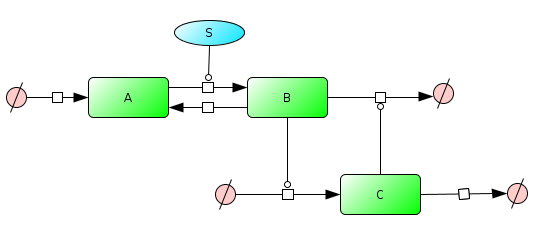
\includegraphics[width=0.8\textwidth]{../figures/model1.png}
            \caption{Topology diagram of model 1.}
            \label{fig:model1:network}
    \end{figure}

    \begin{figure}[t]
        \centering
        \begin{subfigure}{0.45\textwidth}
            \centering
            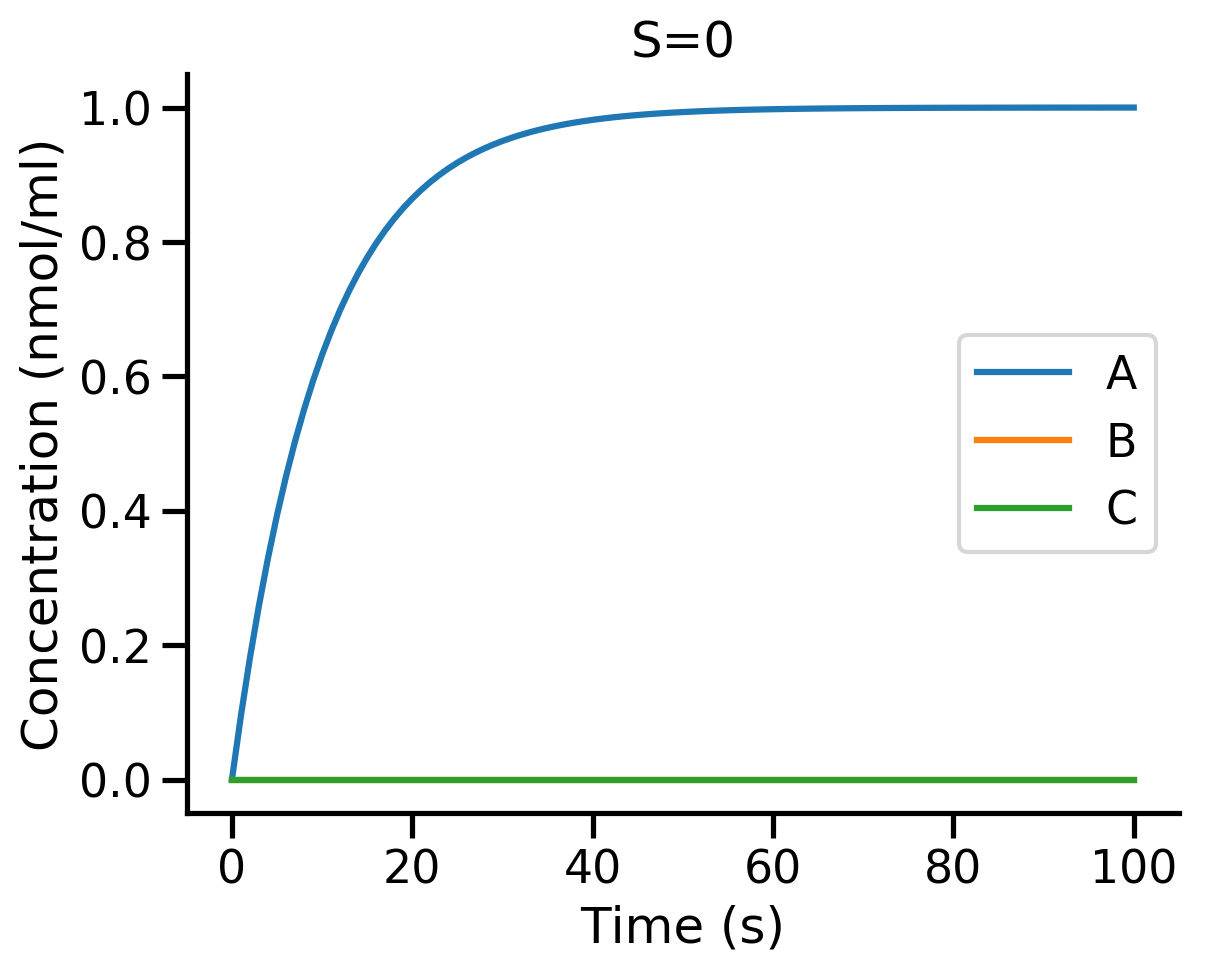
\includegraphics[width=\textwidth]{../figures/WithoutS.png}
            \label{a}
        \end{subfigure}
        \begin{subfigure}{0.45\textwidth}
            \centering
            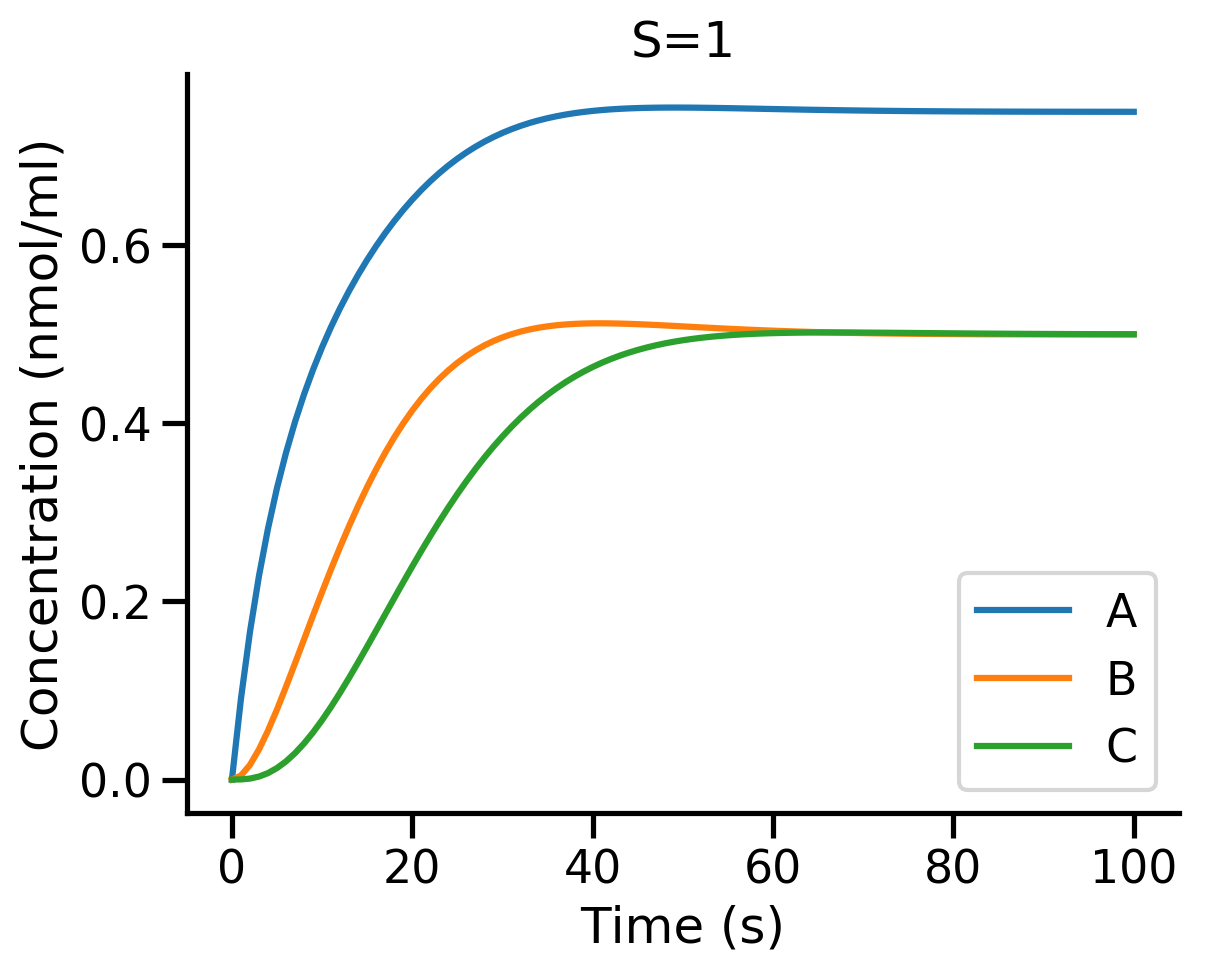
\includegraphics[width=\textwidth]{../figures/WithS.png}}
            \label{b}
        \end{subfigure}
        \caption{Simulation of (a) model 1 with (b) $S_{0}=0$ and (c) $S_0=1$. Initial concentrations: $A=B=C=0$ and
        all kinetic parameters $k_1, ..., k_7 = 0.1$}
        \label{fig:model1}
    \end{figure}

    \begin{enumerate}
        \item Write the model equations with pen and paper
        \item Reproduce the simulation output in \cref{fig:model1} using Copasi
        \item Reproduce the simulation output using tellurium and antimony. The documentation is here (http://tellurium.analogmachine.org/) and there are also some examples in the PyCoTools documentation (https://pycotools3.readthedocs.io/en/latest/)
        \item Change the rate law for the reaction where A gets converted to B by S to michaelis-menten kinetics using both Copasi and Antimony
        \item Change the rate law for the reaction where B is degraded by C to competitive inhibition kinetics using both Copasi and Antimony
        \item Investigate the role of the ki parameter of the competitive inhibition reaction you've just added using both parameter sliders and parameter scans in Copasi
        \item Run a sensitivity analysis in Copasi and try to interpret the results.
    \end{enumerate}

    %    \subsection{}





\end{document}